\documentclass{article}

% 패키지 포함
\usepackage[utf8]{inputenc} % UTF-8 인코딩 지원
\usepackage{amsmath}        % 수식 패키지
\usepackage{graphicx}       % 그림 삽입 패키지
\usepackage{kotex}          % 한글 패키지
\usepackage{float}          % 그림 위치 고정 패키지
\usepackage{listingsutf8}   % listings 패키지의 UTF-8 지원 확장
\usepackage{xcolor}         % 코드 하이라이트 색상 지정용

\lstset{ % 코드 스타일 설정
    inputencoding=utf8,    % 입력 인코딩 설정
    extendedchars=true,    % 확장 문자 지원
    basicstyle=\ttfamily\small, % 기본 글꼴과 크기
    keywordstyle=\color{blue}\bfseries, % 키워드 색상
    commentstyle=\color{green}, % 주석 색상
    stringstyle=\color{red}, % 문자열 색상
    numbers=left, % 줄 번호
    numberstyle=\tiny\color{gray}, % 줄 번호 스타일
    frame=single, % 코드 블록 테두리
    breaklines=true, % 자동 줄바꿈
    language=Python % 코드 언어 설정 (예: Python)
}

\title{Galactic Astronomy: Homework 3}
\author{21010475 신승우}
\date{\today} % 현재 날짜

\begin{document}

\maketitle % 제목 생성

\section{Introduction}

\quad 은하의 light curve는 다음과 같은 de Vaucouleurs profile을 따르는 것으로 알려져 있다.
\begin{equation}
    \mu(r) = \mu_{e}+8.3268\left[\left(\frac{r}{r_{e}}\right)^{1/4}-1\right]
\end{equation}
\quad 그리고 de Vaucouleurs profile의 일반화된 형태인 Sérsic profile은 다음과 같이 주어진다.
\begin{equation}
    \mu(r) = \mu_{e}+8.3268\left[\left(\frac{r}{r_{e}}\right)^{1/n}-1\right]
\end{equation}
\quad 타원은하가 이러한 profile을 따르는지 실제 은하의 Photometry 관측 결과와 
비교해보기 위해 직접 은하 관측을 할 수는 없기 때문에, 
SkyView Virtual Observatory의 DSS Survey data로부터 .fits file을 받아와서 
Mopex 프로그램으로 은하 중심으로부터의 거리에 따른 pixel value data를 구했다.
노이즈를 무시하면 pixel value는 물리적으로 그 pixel에 도달한 photon의 flux에 비례한다. 

\quad Flux density와 magnitude 사이에는 다음과 같은 관계가 성립한다.
\begin{equation}
    m_1-m_2=-2.5\log_{10}\frac{F_1}{F_2}
\end{equation}
$\mu$는 magnitude가 아닌 surface brightness이기 때문에,
\begin{align*}
    \mu(r)-\mu_e&=m(r)-m_e+2.5\log_{10}A-2.5\log_{10}A\\
    &=-2.5\log_{10}\frac{F(r)}{F_e}+2.5\log_{10}\frac{A}{A} \tag{4}\\
    &=-2.5\log_{10}\frac{F(r)}{F_e}
\end{align*}

\quad 정확한 flux density와 pixel value 사이의 관계를 알 수 없기 때문에 
$\mu$ 값을 알아내지는 못했지만, 위 식을 이용해서 $\mu(r)-\mu_e$ 을 계산하여
light curve fitting을 진행했다.

\section{Code}
\begin{lstlisting}
import pandas as pd
import numpy as np
import matplotlib.pyplot as plt
from scipy.optimize import curve_fit
    
galaxy_name = 'your galaxy name'
galaxy = pd.read_csv(
    filepath_or_buffer=f'data/{galaxy_name}.tbl', 
    skiprows=11, 
    sep=r'\s+', 
    names=['Index', 'Lon_LeftReadout', 'Lat_LeftReadout', 'Lon_RightReadout', 'Lat_RightReadout', 'Distance','Flux'],
    index_col=0
)
distance = galaxy['Distance'].to_numpy()
flux = galaxy['Flux'].to_numpy()
flux = np.flip(flux) # if data is fliped

# Masking
mask = distance>50
distance_sorted= distance[mask]
flux_sorted = flux[mask]

r_inner = distance[:-1]  # Inner radii of annuli
r_outer = distance[1:]   # Outer radii of annuli

areas = np.pi * (r_outer**2 - r_inner**2)  # Areas of annuli

d_flux = flux[-1]*areas

# Compute cumulative flux
cumulative_flux = np.cumsum(d_flux)

total_flux = cumulative_flux[-1]

# Find the radius where cumulative flux is half of the total flux
half_flux = total_flux / 2
r_e_index = np.searchsorted(cumulative_flux, half_flux)
r_e = distance[r_e_index]

    
# Compute surface brightness mu(r) = -2.5 * log10(Flux)
# Since Flux_sorted is proportional to surface brightness
mu_r = -2.5 * np.log10(flux/flux[r_e_index-5:r_e_index+5].mean())
mu_r_sorted = mu_r[mask]

# Define the generalized de Vaucouleurs profile function
def deVaucouleurs_profile(r, n):
    return 8.3268 * ((r / r_e) ** (1 / n) - 1)

params, _ = curve_fit(
    f=deVaucouleurs_profile, 
    xdata= distance_sorted,
    ydata= mu_r_sorted,
    p0= 4,
    bounds=((1), (np.inf))
)
n = params[0]
distance_sample = np.linspace(distance[0], distance[-1], 1000)
mu_fit = deVaucouleurs_profile(distance_sample, n)
mu_4 = deVaucouleurs_profile(distance_sample, 4)

print(r_e)

# Plot
fig = plt.figure(figsize=(8, 6))
ax = fig.add_subplot()

ax.scatter(distance, mu_r, s=10)
ax.plot(distance_sample, mu_fit, c='gray', label=f'n={n:.1f}')
ax.plot(distance_sample, mu_4, c='gray', ls='--', label='n=4')


# Details
ax.set_xlim((0, distance.max())); ax.set_ylim((-1.5,0.5))
ax.legend(edgecolor='none')
ax.tick_params(direction='in')
ax.invert_yaxis()  # Invert y-axis because lower magnitudes are brighter
ax.grid(True)

ax.set_title(galaxy_name)
ax.set_xlabel('Distance [arcsec]')
ax.set_ylabel(r'$\mu_{r}-\mu_{e}$ [mag/arcsec$^2$]')

# Save
fig.savefig(f'figures/{galaxy_name}_mu.png')
\end{lstlisting}

\section{Results}
\quad Virgo cluster에 속하는 타원 은하들, M49, M60, M87 은하에 대해서 Sérsic profile fitting을 진행하였다.
아래 그림을 보면 은하의 중심에서 매우 가까운 영역은 flat light curve를 가진다. 
그래서 그 영역은 적절히 제외하고 fitting을 진행한 결과이다.
$x$축은 지구에서 관측한 angular distance이고, $y$축은 $\mu(r)-\mu_{e}$ 값이다.
\begin{figure}[H]
    \centering
    \begin{minipage}{0.45\textwidth}
        \centering
        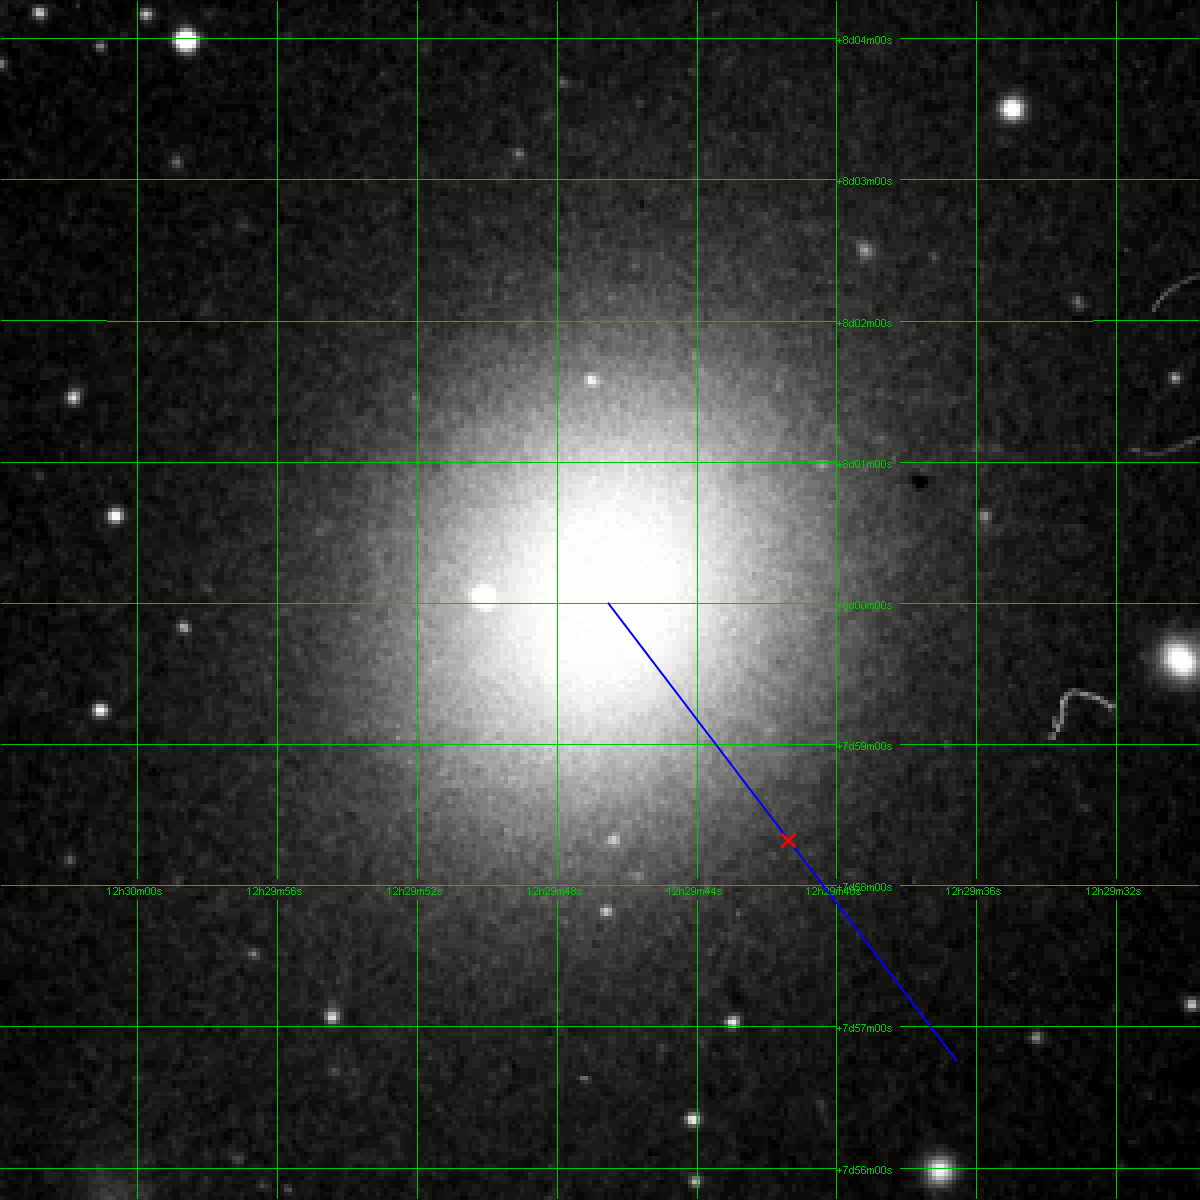
\includegraphics[height=4cm]{figures/M49_image.png} 
        \caption{M49 image}
        \label{fig:M49 image}
    \end{minipage}
    \hfill
    \begin{minipage}{0.45\textwidth}
        \centering
        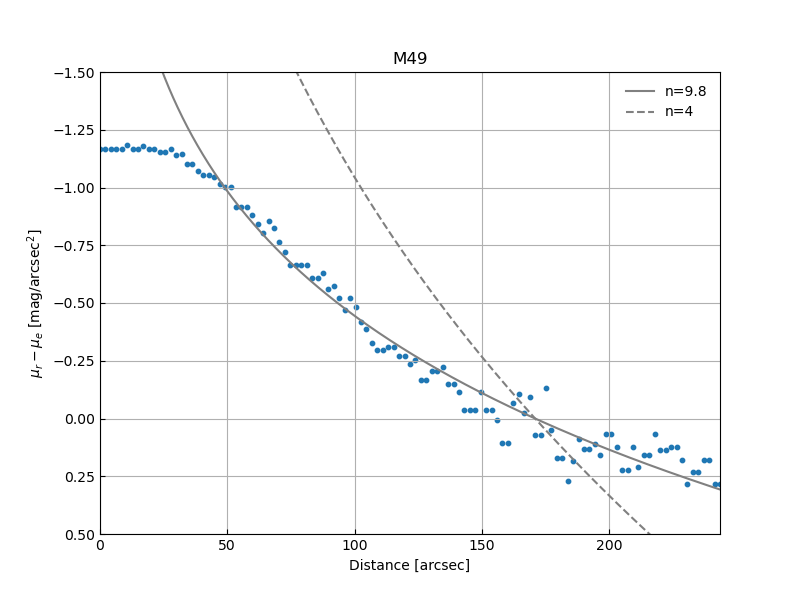
\includegraphics[height=4cm]{figures/M49_mu.png}
        \caption{M49 data}
        \label{fig:M49 data}
    \end{minipage}
\end{figure}

\begin{figure}[H]
    \centering
    \begin{minipage}{0.45\textwidth}
        \centering
        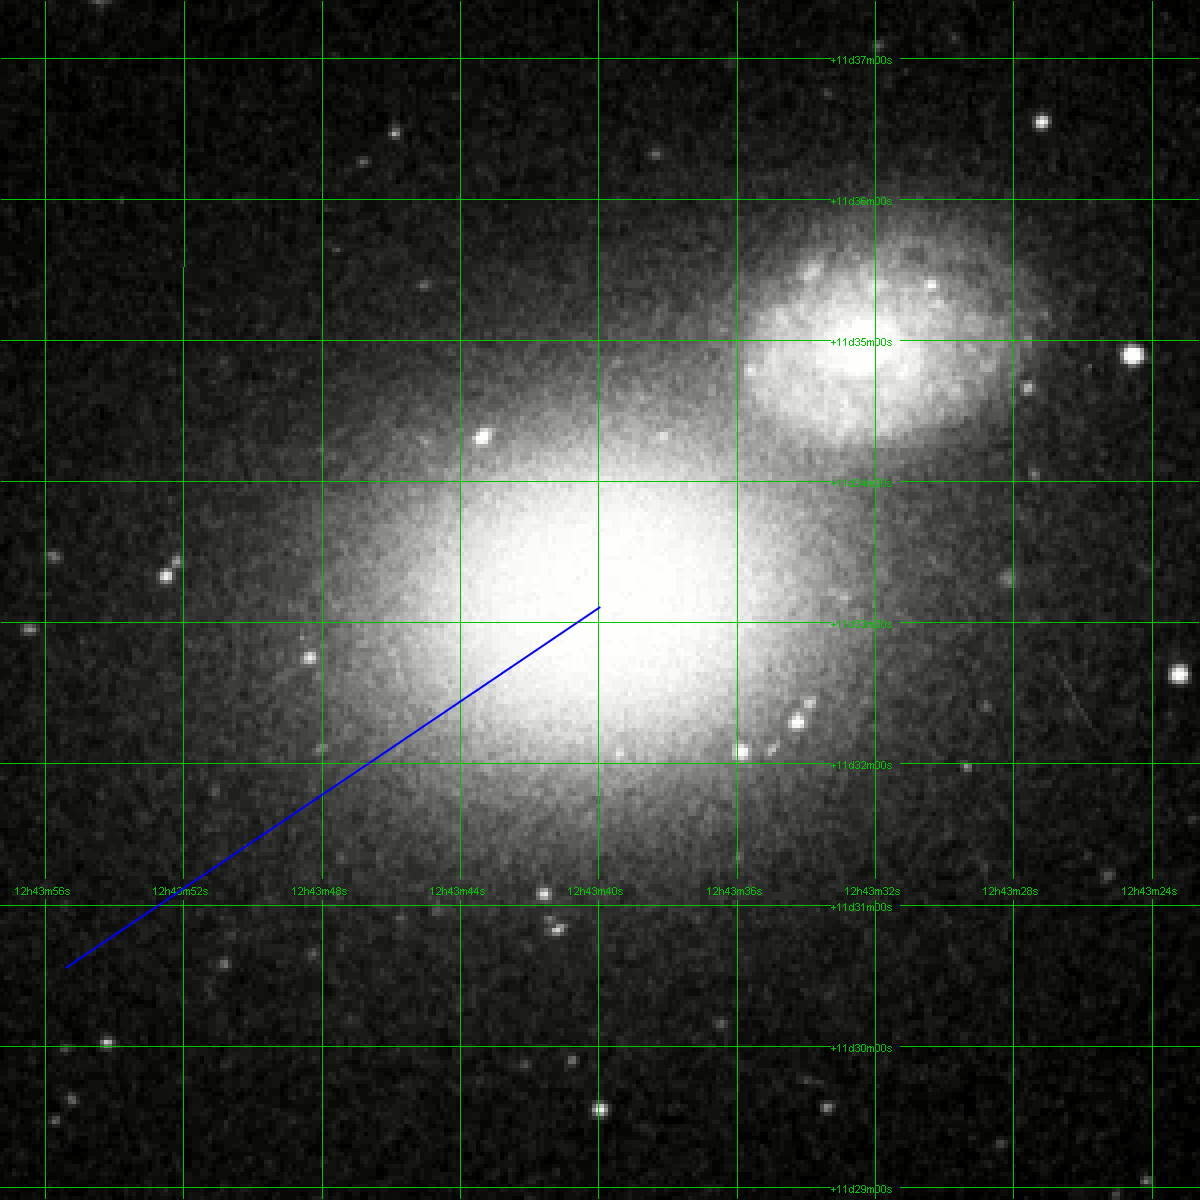
\includegraphics[height=4cm]{figures/M60_image.png} 
        \caption{M60 image}
        \label{fig:M60 image}
    \end{minipage}
    \hfill
    \begin{minipage}{0.45\textwidth}
        \centering
        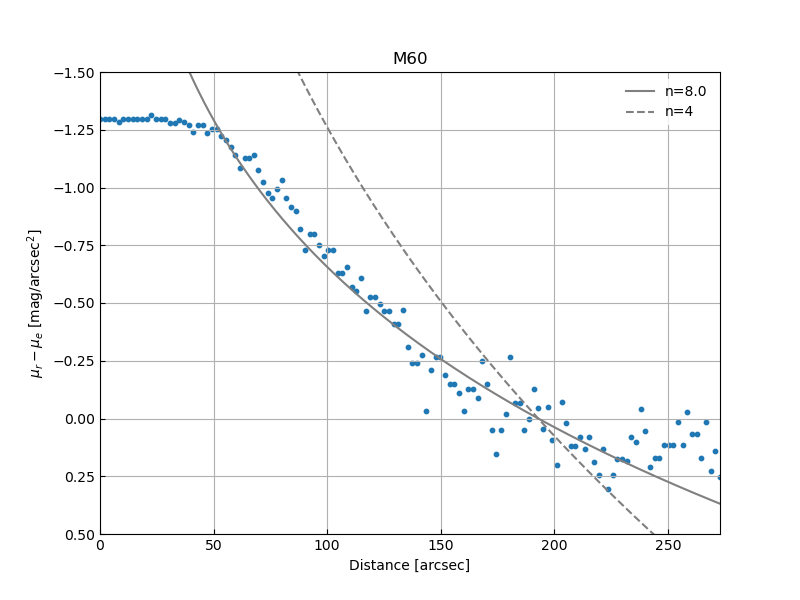
\includegraphics[height=4cm]{figures/M60_mu.png}
        \caption{M60 data}
        \label{fig:M60 data}
    \end{minipage}
\end{figure}

\begin{figure}[H]
    \centering
    \begin{minipage}{0.45\textwidth}
        \centering
        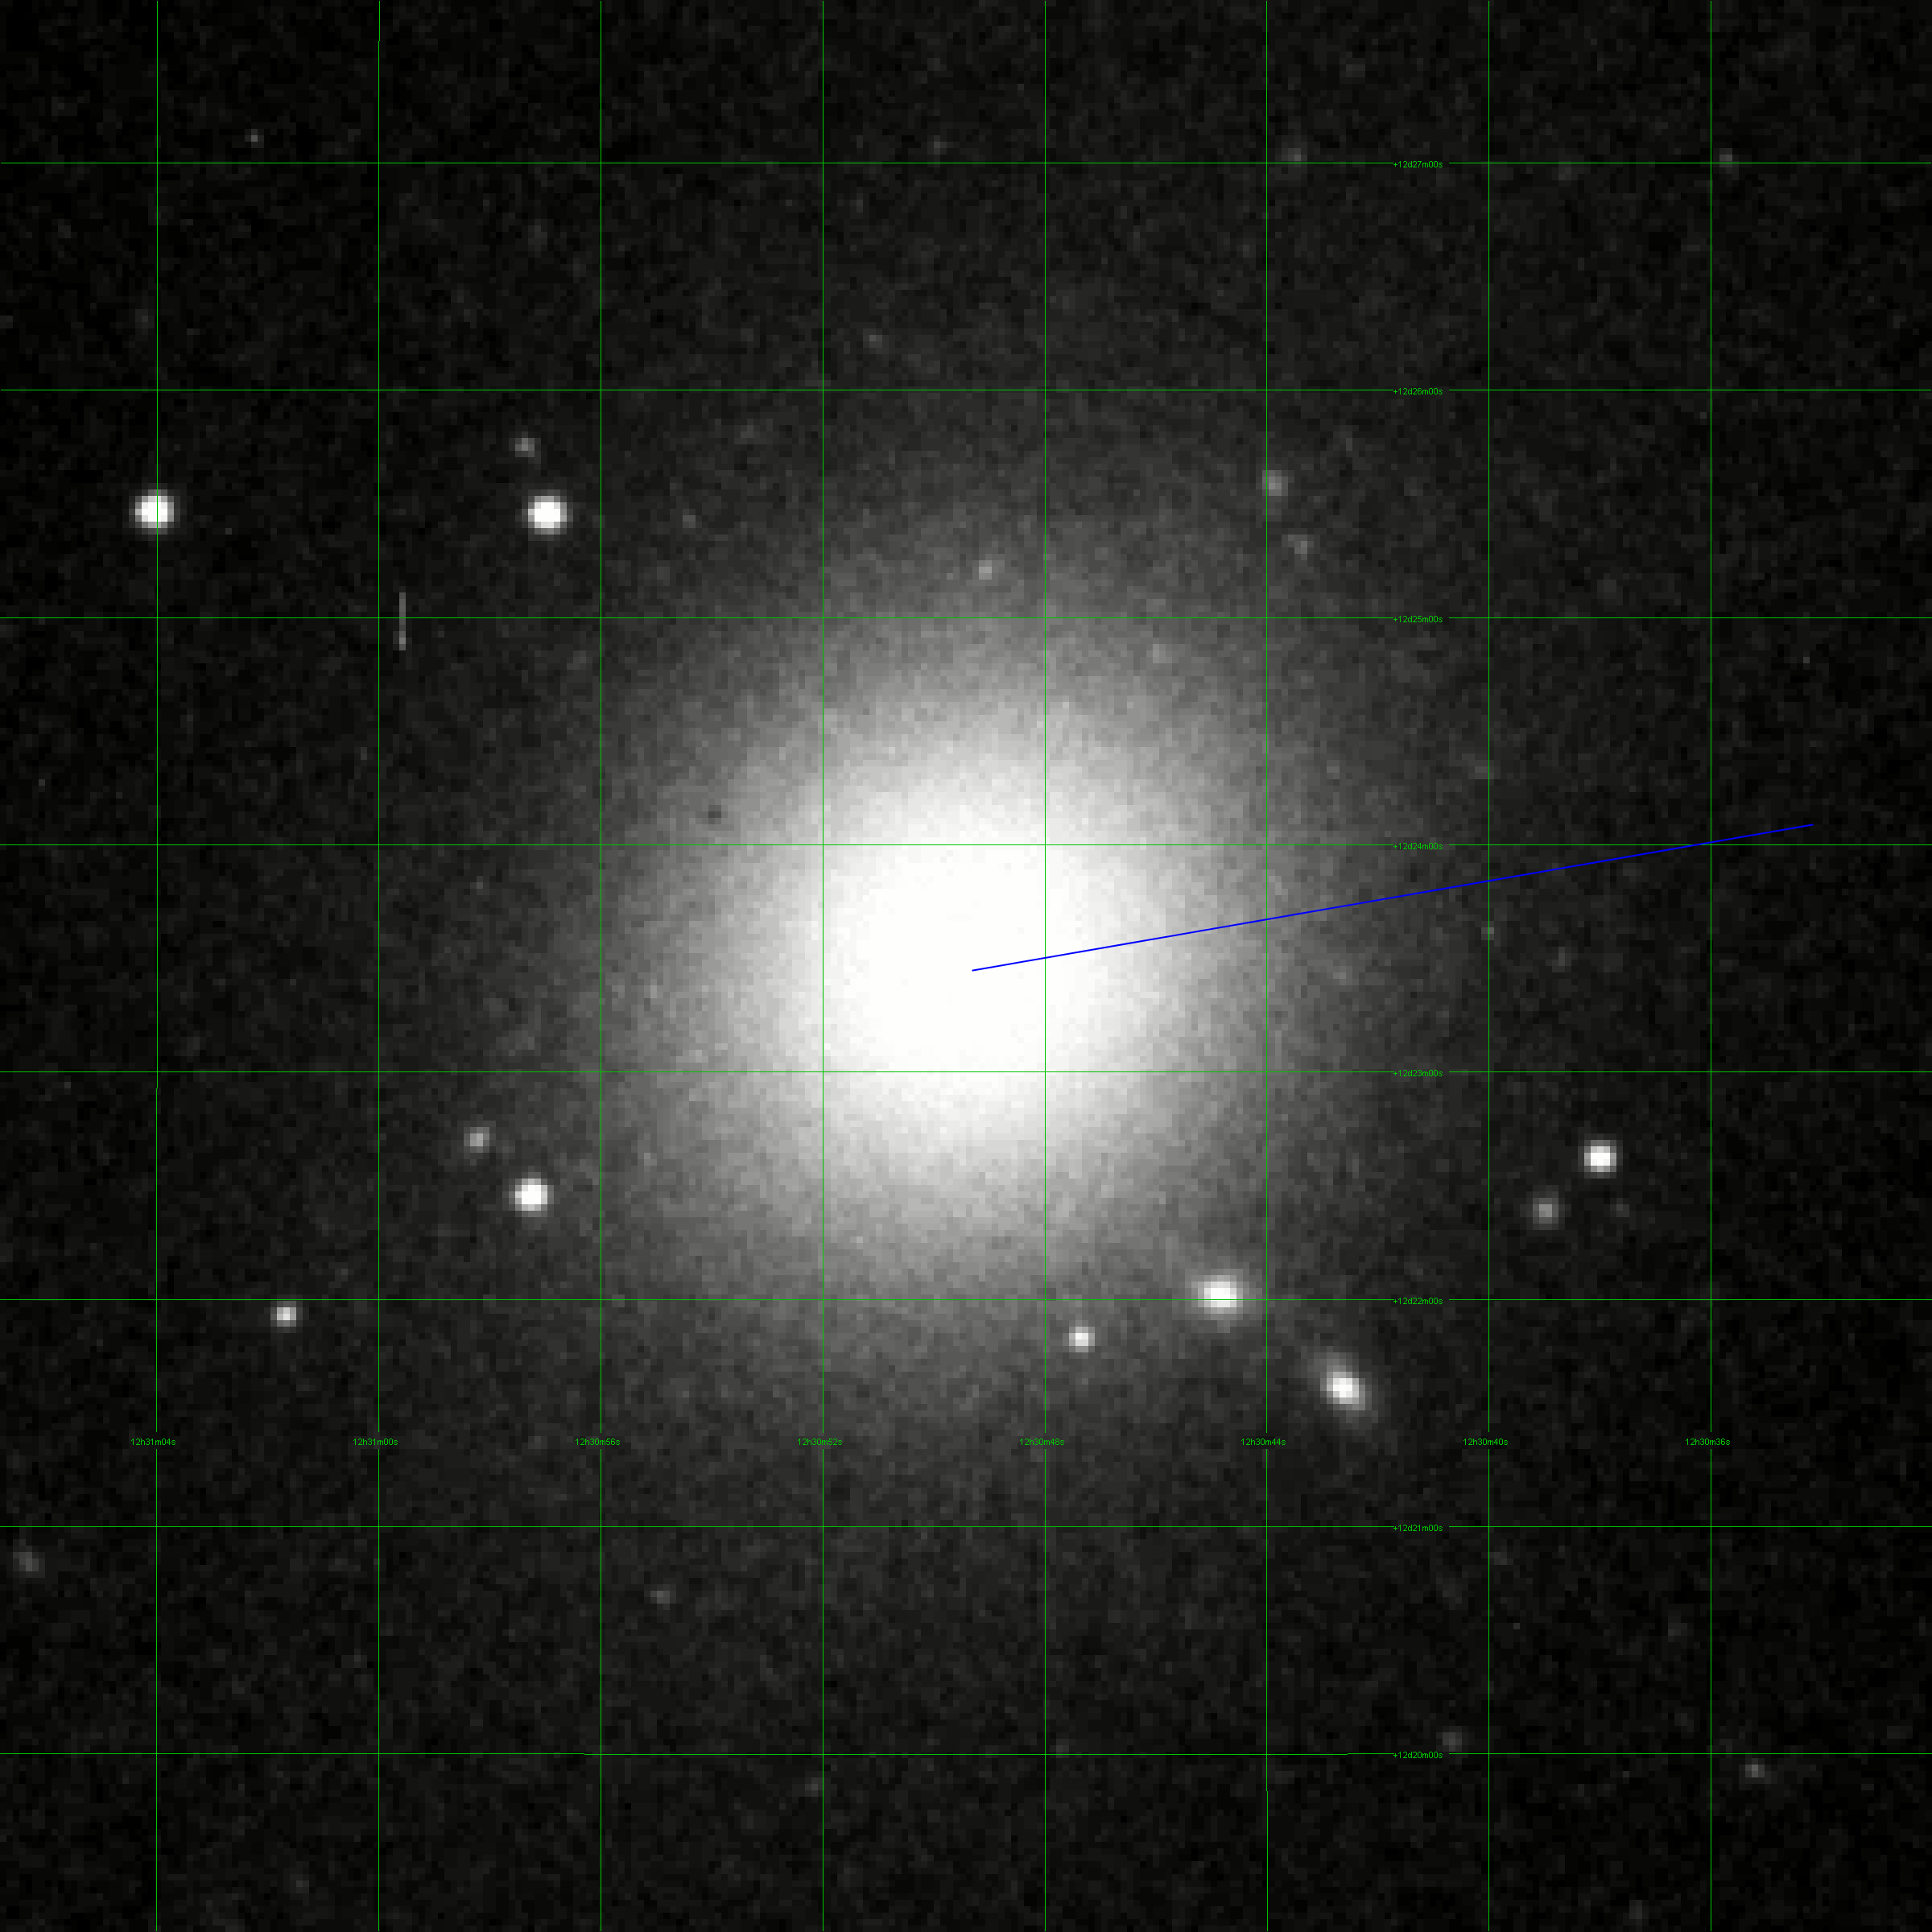
\includegraphics[height=4cm]{figures/M87_image.png} 
        \caption{M87 image}
        \label{fig:M87 image}
    \end{minipage}
    \hfill
    \begin{minipage}{0.45\textwidth}
        \centering
        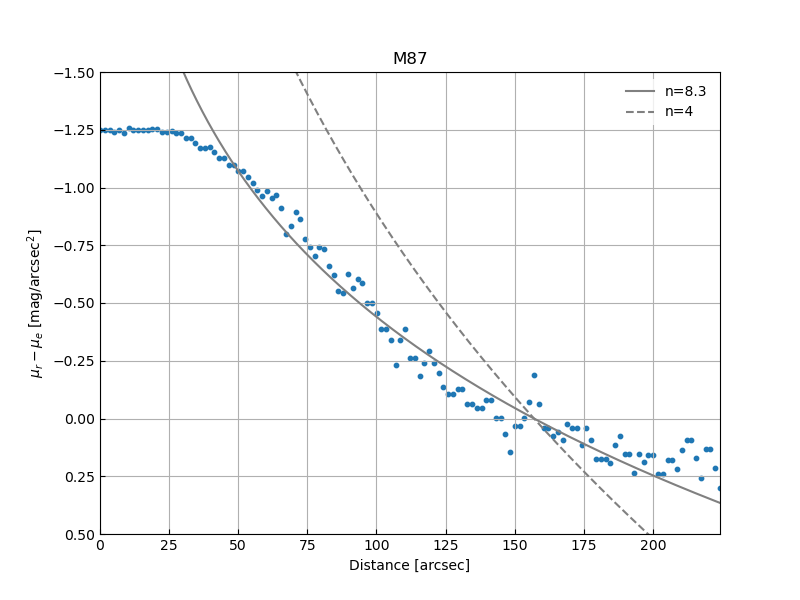
\includegraphics[height=4cm]{figures/M87_mu.png}
        \caption{M87 data}
        \label{fig:M87 data}
    \end{minipage}
\end{figure}

\section{Conclusion}
\quad 그래프를 그려본 결과, 각 타원은하의 light curve는 de Vaucouleurs profile($r^{1/4}$ 법칙)을 따르지 않는다. 
하지만 Sérsic profile($r^{1/n}$ 법칙)을 따른다고 가정하고 curve fitting을 했을 때는 light curve가 잘 fitting이 된다.
따라서 M49, M60, M87은하의 light curve는 Sérsic profile을 따르는 것으로 보인다.
\end{document}
